% The following section and subsections reuse the work done in the Distributed Systems Seminar, during the fall semester of the 2022/2023 academic year. The original version of the seminar paper can be found in \cite{units-of-permissionless-consensus}.

Long has been the time when consensus was still on the verge of being considered such a fundamental problem of distributed systems. Generally defined by Lamport et al. \cite{pease1980reaching, lamport2019byzantine}, consensus means reaching an agreement between multiple parties in the potential presence of faulty individuals. As per multi-agent systems, interacting over computer networks, consensus is thought to be the result of a coordination effort, that eventually leads the parties to agree on some value at a given moment. However, the evolution of the consensus problem has been invariably limited by a set of strong assumptions. The well-known Byzantine-Fault-Tolerant multiparty consensus systems, that have been designed over the years, are usually meant to work only with a set of known participants, being them faulty or not \cite{castro1999practical}. 

The other side of the coin is the permissionless consensus challenge, consisting of achieving agreement in an environment where the parties are unknown and untrusted \cite{nakamoto2008bitcoin, buterin2014next}. The relative openness and lack of any kind of central authority are other intrinsic particularities of this type of networks, which inevitably adds complexity to the problem. The participants are not only unknown and untrusted but can also join or leave the network at any time, freely choosing if they care to participate in the consensus protocol. Nevertheless, the problem of permissionless consensus is still seen as a special case of the general consensus definition, but under more meticulous trust assumptions.

Further in this thesis, we will evaluate the different high-level \pol{} protocols and draw a parallel between the evolution of their trust levels and the ultimate need for a low-level permissionless consensus algorithm that allows for establishing decentralized and time-conscious agreement, in an eventual trustless setup, between the multiple witnesses. The next subsections will briefly review some of the most relevant aspects and proof units that give practicality to the roots of the permissionless consensus problem.

\subsubsection{Proof-of-X}

The solution is, nonetheless, unsettled and the scientific community has been reasoning about the need for permissionless consensus when there are already well known and established consensus protocols that work in trusted environments \cite{castro1999practical, miller2016honey}. However, even those protocols have their own limitations, not only in terms of trust, fault-tolerance, centrality, permissions, or bottlenecks, but also in terms of scalability \cite{miller2016honey}, despite assuring deterministic finality \cite{decker2016bitcoin}. The need for permissionless consensus is then justified by the fact that permissioned protocols are not compatible with the requirements of the new generation of distributed systems, especially in the context of Blockchain networks. These requirements include dealing with today's sparse networks of anonymously and dynamically participating devices, without interrupting consensus and while battling the disruption of the system, typically by subverting it with many pseudo-entities~\textemdash~the so-called Sybil attacks \cite{8629877, survey-dist-consensus}. Fundamentally, the permissionless consensus problem is the need for a consensus protocol that can be run in a distributed and decentralized environment, where the participants are unknown and untrusted, and where the network is bigger, sparser and unpredictably less reliable.

Technically, permissionless environments allow for larger networks that depict lower connectivity between the participants. Operationally, everything is expected to happen in an asynchronous or partially synchronous fashion, and the number of transactions is predicted to be smaller than in the permissioned counterparts. Participation is free, and the governance is not centralized, but rather distributed and public. The identity of the participants is secured or semi-secured as it often relies on pseudonymity for protecting the nodes' identity, enabling, at the same time, full transparency concerning the rest of the network's content and operation \cite{xiao2019distributed}. Expectedly, the goal of permissionless consensus, as for any consensus protocol, is to reach agreement on a single value, or a set of values. However, due to the nature of the protocols, the values that are agreed upon end up establishing the serialization of the transactions, and so establishing time consciousness and total order of the events \cite{8629877}.

\begin{figure}[ht]
  \begin{center}
  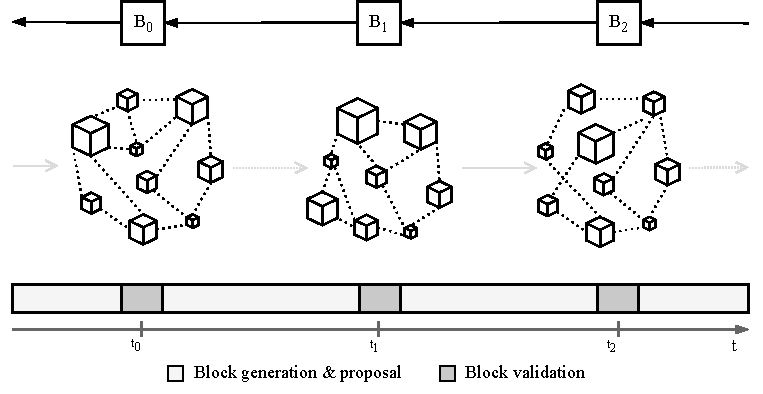
\includegraphics[width=0.9\textwidth]{building-blocks-consensus.pdf}
  \caption{An illustration of the permissionless consensus building phases. From the bottom to the top, the asymmetric arrow of time discretizes the block generation and proposal phases, followed by the block validation, along with frequent network topology changes and the consequent time conscious serialization of the blocks.}
  \label{fig:building-blocks-consensus}
  \end{center}
\end{figure}

Also described by Xiao et al. \cite{survey-dist-consensus}, very concisely, the way to achieve an operating protocol, as seen in the mainstream Blockchain networks, is by first generating the agreeable value, in this particular case, a block and its proof, proposing and disseminating the information to the network, followed by the eventual validation and acceptance of the block by the majority of the nodes. This is the approximate moment of probabilistic finality, when consensus is ultimately reached (see Figure~\ref{fig:building-blocks-consensus}). During the whole process, a fair and somewhat predictable incentive mechanism is also needed, that rewards participants for their honest effort in reaching consensus, and punishes the ones that are not behaving correctly. These incentives are of major importance in this very context of permissionless consensus and all these building phases form the basis of the inner functioning of Bitcoin itself \cite{nakamoto2008bitcoin}, replicated with some variations in other networks \cite{buterin2014next, survey-dist-consensus}. The following is a short introduction to some relevant proof units that feature in the most popular Blockchain systems.

\subsubsection{Proof-of-Work and Proof-of-Stake}

Without discrediting the previous attempts, the first practical permissionless consensus algorithm was proposed by Nakamoto in \cite{nakamoto2008bitcoin}. It is a Proof-of-Work consensus protocol that resembles a replicated state machine where the independent participants reach agreement not only about transactional values, but also about their order - naturally forming the underlying structure of what is now known as a Blockchain. The focus shifted for decentralized systems and after Proof-of-Work many other consensus mechanisms have been proposed, relying on different consensus units.

In the classical Nakamoto consensus protocol, the generation of a block, to be proposed for further network agreement, complies with the unit of computational work needed to create, or rather find, a verifiable proof of the effort spent on assembling the block \cite{nakamoto2008bitcoin}. This essentially requires brute forcing the search for a cryptographic hash value for the aggregation of the block information with a nonce. This value has to satisfy a difficulty threshold (see Procedure \ref{proc:BlockGeneration}), which gets adjusted dynamically over time, to maintain the network overall requirement for the block generation interval \cite{8629877, survey-dist-consensus}.

\begin{procedure} [!h]
	\caption{BlockGeneration()} \label{proc:BlockGeneration}
	\KwIn{Transaction Merkel Tree Root, Hash of the last Block, Timestamp, Other.}
	\KwResult{new $Block$.}
	\BlankLine
  $BlockHeader \ \gets$ Transaction Merkle Tree Root
  \\ \qquad $| \ $ Hash of the last Block
  \\ \qquad $| \ $ Timestamp
  \\ \qquad $| \ $ Other\;
  \BlankLine
  \tcp{the preceding zero bits in $target$ depict the mining difficulty}
  \While{$Hash(BlockHeader \ | \ nonce) \geq target$}{
    Increment $nonce$\;
  }
  \tcp{append transactional data}
  \Return new $Block$\;
	%\eIf{error messages were found}{\Return \False\;}{\Return \True\;}
\end{procedure}

One can then exercise the reasoning line and extrapolate the previous block generation mechanism to a \emph{Proof-of-Something} pseudo-random competition in which an entity in possession of a higher amount of a certain resource, either computational power, or stake, or certain currency, or, for instance, a higher amount of storage space, guarantees a higher probability of leading the block generation and proposal, and consequently winning the acceptance by the majority. This is the essence of Proof-of-Stake, as a derivative of the Proof-of-Work mechanism. Here, stake is a traceable and verifiable amount of a certain unit, token or currency, that is owned by a certain entity who wishes to participate in the consensus protocol. The stake works as a form of collateral that is used to guarantee everyone's honesty, in an attempt to reduce the Sybil attack likelihood. And, respectively as in Proof-of-Work with computational power, the higher the stake, the higher the probability of leading the block generation and proposal.

Idealized and inspired by Proof-of-Stake, extending or adapting Proof-of-Work became a popular trend in the Blockchain community. The main idea is to replace the computational power with some other resource, that is more scarce, or more valuable, or more verifiable, or more traceable, to combine multiple resources, or even to add extra requirements to pure Proof-of-Work \cite{survey-dist-consensus}. Not that every one of the options has a considerable potential for entirely solving the permissionless consensus problem, but each one of them may tackle different use cases where consensus needs to be reached, and where different resources are available to make the agreement happen \cite{BOURAGA2021114384, 9376868}. Nonetheless, the design of these consensus mechanisms shall aim for a protocolar choice between a set of properties that form a trilemma: security, scalability, and decentralization. Briefly put, relaxing the security requirements may allow for more scalability, both of which, consequently, have hands tied with decentralization. These trade-offs are of practical consideration when defining the network goals and use cases \cite{survey-dist-consensus}. Further dissection of various classes of Proof-of-Stake based protocols, diverging alternatives to the classic Nakamoto consensus, and comparisons between them can be found in \cite{8629877, survey-dist-consensus, BOURAGA2021114384, 9376868, natoli2019deconstructing}.

With all the above in mind, we will proceed to review some of the proposed \pol{} solutions, discriminated by trust levels. Aiming at achieving spatio-temporal agreement among the witnesses, we will reason about the applicability of one of these lower-level permissionless consensus protocols, in the context of a fully decentralized and trustless environment.